\documentclass{article}

\usepackage{fancyhdr}
\usepackage{extramarks}
\usepackage{amsmath}
\usepackage{amsthm}
\usepackage{bm}
\usepackage{amsfonts}
\usepackage{tikz}
\usepackage[plain]{algorithm}
\usepackage{algpseudocode}
\usepackage{geometry}

\usetikzlibrary{automata,positioning}


%%%%%%%%%%%%%%%%%%%%%%%%%%%%%%%%%%%%%%%%%%%%%%%%%%%%%%%%%%%%%%%%%%%%%%%%%%%%%%%%%%%%%%%%%
% Basic Document Settings
%%%%%%%%%%%%%%%%%%%%%%%%%%%%%%%%%%%%%%%%%%%%%%%%%%%%%%%%%%%%%%%%%%%%%%%%%%%%%%%%%%%%%%%%%

%%% Page Size %%%
\geometry{
    a4paper,
    % total={170mm,257mm},
    % left=20mm,
    % top=20mm,
}
\voffset=0mm
\topmargin=-10mm
\textheight=245mm
\headsep=7mm
\footskip=11mm

\hoffset=0mm
\textwidth=159.2mm
\evensidemargin=0mm
\oddsidemargin=0mm

\linespread{1.1}
\setlength\parindent{0mm}
\setlength\parskip{10pt}
\allowdisplaybreaks

%%% Header & Footer %%%
\pagestyle{fancy}
% \lhead{\hmwkAuthorName}
\lhead{\hmwkClass\ \hmwkTitle}
% \rhead{\firstxmark}
\rhead{}
% \lfoot{\lastxmark}
\cfoot{Page | \thepage}
\renewcommand\headrulewidth{0.4pt}
\renewcommand\footrulewidth{0.4pt}

%%% Font %%%
\renewcommand{\familydefault}{\sfdefault}
% \renewcommand{\familydefault}{\rmdefault}


%%%%%%%%%%%%%%%%%%%%%%%%%%%%%%%%%%%%%%%%%%%%%%%%%%%%%%%%%%%%%%%%%%%%%%%%%%%%%%%%%%%%%%%%%
% Homework Details
%   - Title
%   - Due date
%   - Class
%   - Section/Time
%   - Instructor
%   - Author
%   - Updated Date
%%%%%%%%%%%%%%%%%%%%%%%%%%%%%%%%%%%%%%%%%%%%%%%%%%%%%%%%%%%%%%%%%%%%%%%%%%%%%%%%%%%%%%%%%
\newcommand{\hmwkTitle}{Assignment \#3 - Written Part}
\newcommand{\hmwkDueDate}{}
\newcommand{\hmwkClass}{Stanford CS224n (2023)}
\newcommand{\hmwkClassTime}{}
\newcommand{\hmwkClassInstructor}{}
\newcommand{\hmwkAuthorName}{\textbf{}}
\newcommand{\hmwkUpdateDate}{2\textsuperscript{nd} March, 2023}


%%%%%%%%%%%%%%%%%%%%%%%%%%%%%%%%%%%%%%%%%%%%%%%%%%%%%%%%%%%%%%%%%%%%%%%%%%%%%%%%%%%%%%%%%
% Title Page
%%%%%%%%%%%%%%%%%%%%%%%%%%%%%%%%%%%%%%%%%%%%%%%%%%%%%%%%%%%%%%%%%%%%%%%%%%%%%%%%%%%%%%%%%
\title{
    \vspace{2in}
    % \textmd{\textbf{\hmwkClass:\ \hmwkTitle}}\\
    % \normalsize\vspace{0.1in}\small{Due\ on\ \hmwkDueDate}\\
    \vspace{0.1in}\large{\textit{\hmwkClassInstructor\ \hmwkClassTime}}
    \vspace{3in}
}

\author{\hmwkAuthorName}
\date{}


%%%%%%%%%%%%%%%%%%%%%%%%%%%%%%%%%%%%%%%%%%%%%%%%%%%%%%%%%%%%%%%%%%%%%%%%%%%%%%%%%%%%%%%%%
% Create Problem Sections and Problem Environment
%
% This environment takes an optional argument. When given, it will adjust the
% problem counter. This is useful for when the problems given for your
% assignment aren't sequential. See the last 3 problems of this template for an
% example.
%%%%%%%%%%%%%%%%%%%%%%%%%%%%%%%%%%%%%%%%%%%%%%%%%%%%%%%%%%%%%%%%%%%%%%%%%%%%%%%%%%%%%%%%%
\newcommand{\hmwkSectionPrefix}{Question }
% \newcommand{\hmwkSectionPrefix}{Problem }

\newcommand{\hmwkSectionIndex}{\alph}
% \newcommand{\hmwkSectionIndex}{\arabic}

\newcommand{\hmwkSectionText}{\hmwkSectionPrefix (\hmwkSectionIndex{homeworkProblemCounter})}

\newcommand{\enterProblemHeader}[1]{
    \nobreak\extramarks{\hmwkSectionPrefix (\hmwkSectionIndex{#1}) continued on next page\ldots}\nobreak{}
    \nobreak\extramarks{\hmwkSectionPrefix (\hmwkSectionIndex{#1}) (continued)}{\hmwkSectionPrefix (\hmwkSectionIndex{#1}) continued on next page\ldots}\nobreak{}
}

\newcommand{\exitProblemHeader}[1]{
    \nobreak\extramarks{\hmwkSectionPrefix (\hmwkSectionIndex{#1}) (continued)}{\hmwkSectionPrefix (\hmwkSectionIndex{#1}) continued on next page\ldots}\nobreak{}
    \stepcounter{#1}
    \nobreak\extramarks{\hmwkSectionPrefix (\hmwkSectionIndex{#1})}{}\nobreak{}
}

\setcounter{secnumdepth}{0}
\newcounter{partCounter}
\newcounter{homeworkProblemCounter}
\setcounter{homeworkProblemCounter}{1}
\nobreak\extramarks{\hmwkSectionPrefix (\hmwkSectionIndex{homeworkProblemCounter})}{}\nobreak{}

\newenvironment{homeworkProblem}[1][-1]{
    \ifnum#1>0
        \setcounter{homeworkProblemCounter}{#1}
    \fi
    \section{\hmwkSectionText}
    \setcounter{partCounter}{1}
    \enterProblemHeader{homeworkProblemCounter}
}{
    \exitProblemHeader{homeworkProblemCounter}
}


%%%%%%%%%%%%%%%%%%%%%%%%%%%%%%%%%%%%%%%%%%%%%%%%%%%%%%%%%%%%%%%%%%%%%%%%%%%%%%%%%%%%%%%%%
% Various Helper Commands
%%%%%%%%%%%%%%%%%%%%%%%%%%%%%%%%%%%%%%%%%%%%%%%%%%%%%%%%%%%%%%%%%%%%%%%%%%%%%%%%%%%%%%%%%
\renewcommand{\part}[1]{\textbf{Part \alph{partCounter}}\stepcounter{partCounter}\\}

% Useful for algorithms
\newcommand{\alg}[1]{\textsc{\bfseries \footnotesize #1}}

% For derivatives
\newcommand{\deriv}[1]{\frac{\mathrm{d}}{\mathrm{d}x} (#1)}

% For partial derivatives
\newcommand{\pderiv}[2]{\frac{\partial}{\partial #1} (#2)}

% Integral dx
\newcommand{\dx}{\mathrm{d}x}

% Alias for the Solution section header
\newcommand{\solution}{\textbf{\large Solution}}

% Probability commands: Expectation, Variance, Covariance, Bias
\newcommand{\E}{\mathrm{E}}
\newcommand{\Var}{\mathrm{Var}}
\newcommand{\Cov}{\mathrm{Cov}}
\newcommand{\Bias}{\mathrm{Bias}}


%%%%%%%%%%%%%%%%%%%%%%%%%%%%%%%%%%%%%%%%%%%%%%%%%%%%%%%%%%%%%%%%%%%%%%%%%%%%%%%%%%%%%%%%%
% Main Document
%%%%%%%%%%%%%%%%%%%%%%%%%%%%%%%%%%%%%%%%%%%%%%%%%%%%%%%%%%%%%%%%%%%%%%%%%%%%%%%%%%%%%%%%%
\begin{document}
% \maketitle
% \pagebreak
{Updated on: \hmwkUpdateDate}

\vspace{1em}

\textbf{\Large 1 Machine Learning \& Neural Networks}

\begin{homeworkProblem}

    \textbf{Part (i)}

    In each step $t$, parameters ${\theta_t}$ are updated along the direction
    of momemtum $\bm{m_{t+1}}$ in the next step, which is a weight mean between
    momentum $\bm{m_t}$ and gradient $\nabla_{\theta_t} J(\theta_t)$ of the
    current step. Here, the momentum takes a much higher weight (usually 90\%)
    and so a large proportion of previous direction is preserved. The change in
    each update direction (fluctuation) is reduced and hence achieving a higher
    rate of convergence towards the minima.

    \textbf{Part (ii)}

    $\bm{v_t}$ keeps track of the rolling average of the magnitude of gradients
    in each step. For parameters having small gradients, the corresponding
    momentums are divided by smaller $\bm{v_t}$ elements and hence the
    parameters get boosted updates. On the other hands, parameters with
    frequent updates are divided by a larger $\bm{v_t}$ and therefore update
    with smallers steps. The bias towards parameters in the learning process is
    reduced.

\end{homeworkProblem}

\begin{homeworkProblem}

    \textbf{Part (i)}

    \begin{align*}
        \E_{P_{drop}}[\bm{h}_{drop}]_i &= h_i \\
        \E_{P_{drop}}[\lambda\bm{d} \odot \bm{h}]_i &= h_i \\
        \E_{P_{drop}}[d_i] \times \lambda h_i &= h_i \\
        (1 - p_{drop}) \times \lambda h_i &= h_i \\
        \lambda &= \frac{1}{1-p_{drop}}
    \end{align*}

    \textbf{Part (ii)}

    In the training process, dropout should be adopted to prevent overfitting
    the model on the training data. When overfitting occurs, some neurons
    dominate the model output. When dominated neurons are turned off randomly,
    other neurons are forced to learn other hidden patterns from the training
    data. Thus, all neurons are trained to contribute to the model output based
    on different aspects of the input. Dropout should therefore not be used
    during evaluation such that all neurons are involved in affecting the model
    output.

\end{homeworkProblem}

\pagebreak

\textbf{\Large 2 Neural Transition-Based Dependency Parsing}

\begin{homeworkProblem}[1]
    \noindent\makebox[\textwidth]{
        \begin{tabular}{ l | l | l | l}
            Stack & Buffer & New dependency & Transition \\ \hline
            [ROOT] & [I, attended, lectures, in, the, NLP, class] &  & Initial Configuration \\
            $[$ROOT, I] & [attended, lectures, in, the, NLP, class] &  &  \texttt{SHIFT}  \\
            $[$ROOT, I, attended] & [lectures, in, the, NLP, class] &  &  \texttt{SHIFT}  \\
            $[$ROOT, attended] & [lectures, in, the, NLP, class] & attended$\to$I &  \texttt{LEFT-ARC}  \\
            $[$ROOT, attended, lectures] & [in, the, NLP, class] &  &  \texttt{SHIFT}  \\
            $[$ROOT, attended] & [in, the, NLP, class] & attended$\to$lectures &  \texttt{RIGHT-ARC}  \\
            $[$ROOT, attended, in] & [the, NLP, class] &  &  \texttt{SHIFT}  \\
            $[$ROOT, attended, in, the] & [NLP, class] &  &  \texttt{SHIFT}  \\
            $[$ROOT, attended, in, the, NLP] & [class] &  &  \texttt{SHIFT}  \\
            $[$ROOT, attended, in, the, NLP, class] & [ ] &  &  \texttt{SHIFT}  \\
            $[$ROOT, attended, in, the, class] & [ ] & class$\to$NLP &  \texttt{LEFT-ARC}  \\
            $[$ROOT, attended, in, class] & [ ] & class$\to$the &  \texttt{LEFT-ARC}  \\
            $[$ROOT, attended, class] & [ ] & class$\to$in &  \texttt{LEFT-ARC}  \\
            $[$ROOT, attended] & [ ] & attended$\to$class &  \texttt{RIGHT-ARC}  \\
            $[$ROOT] & [ ] & ROOT$\to$attended &  \texttt{RIGHT-ARC}  \\
        \end{tabular}
    }
\end{homeworkProblem}

\begin{homeworkProblem}
    One step is required to shift each word to the stack from the buffer. An
    extra step is then required to move each word out of the stack to create
    a dependency. Therefore, $2n$ steps are required.
\end{homeworkProblem}

\begin{homeworkProblem}[5]
    dev UAS: 87.43\\
    test UAS: 87.64
    \begin{figure}[h]
        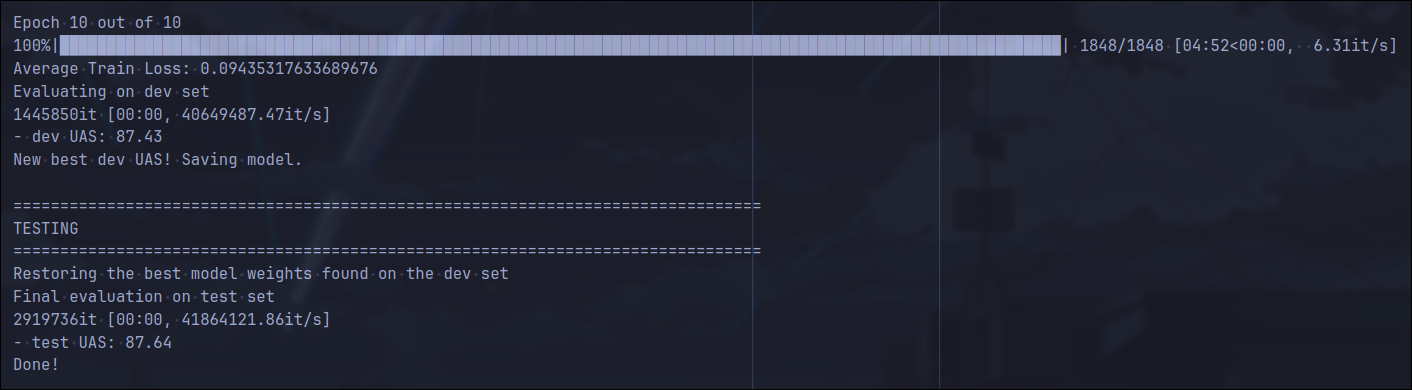
\includegraphics[width=15cm]{a3_written_training_result.png}
        \centering
    \end{figure}
\end{homeworkProblem}

\newpage

\begin{homeworkProblem}
    \textbf{Part (i)}
    \begin{description}
        \item[Error type:] Verb Phrase Attachment Error
        \item[Incorrect dependency:] acquisition $\to$ citing
        \item[Correct dependency:] blocked $\to$ citing
     \end{description}

    \textbf{Part (ii)}
    \begin{description}
        \item[Error type:] Modifier Attachment Error
        \item[Incorrect dependency:] left $\to$ early
        \item[Correct dependency:] afternoon $\to$ early
    \end{description}

    \textbf{Part (iii)}
    \begin{description}
        \item[Error type:] Prepositional Phrase Attachment Error
        \item[Incorrect dependency:] declined $\to$ decision
        \item[Correct dependency:] reasons $\to$ decision
    \end{description}

    \textbf{Part (iv)}
    \begin{description}
        \item[Error type:] Coordination Attachment Error
        \item[Incorrect dependency:] affects $\to$ one
        \item[Correct dependency:] plants $\to$ one
    \end{description}
\end{homeworkProblem}


\end{document}
